\PassOptionsToPackage{unicode=true}{hyperref} % options for packages loaded elsewhere
\PassOptionsToPackage{hyphens}{url}
%
\documentclass[]{article}
\usepackage{lmodern}
\usepackage{amssymb,amsmath}
\usepackage{ifxetex,ifluatex}
\usepackage{fixltx2e} % provides \textsubscript
\ifnum 0\ifxetex 1\fi\ifluatex 1\fi=0 % if pdftex
  \usepackage[T1]{fontenc}
  \usepackage[utf8]{inputenc}
  \usepackage{textcomp} % provides euro and other symbols
\else % if luatex or xelatex
  \usepackage{unicode-math}
  \defaultfontfeatures{Ligatures=TeX,Scale=MatchLowercase}
\fi
% use upquote if available, for straight quotes in verbatim environments
\IfFileExists{upquote.sty}{\usepackage{upquote}}{}
% use microtype if available
\IfFileExists{microtype.sty}{%
\usepackage[]{microtype}
\UseMicrotypeSet[protrusion]{basicmath} % disable protrusion for tt fonts
}{}
\IfFileExists{parskip.sty}{%
\usepackage{parskip}
}{% else
\setlength{\parindent}{0pt}
\setlength{\parskip}{6pt plus 2pt minus 1pt}
}
\usepackage{hyperref}
\hypersetup{
            pdftitle={MLR Examples},
            pdfauthor={SDS 291},
            pdfborder={0 0 0},
            breaklinks=true}
\urlstyle{same}  % don't use monospace font for urls
\usepackage[margin=1in]{geometry}
\usepackage{color}
\usepackage{fancyvrb}
\newcommand{\VerbBar}{|}
\newcommand{\VERB}{\Verb[commandchars=\\\{\}]}
\DefineVerbatimEnvironment{Highlighting}{Verbatim}{commandchars=\\\{\}}
% Add ',fontsize=\small' for more characters per line
\usepackage{framed}
\definecolor{shadecolor}{RGB}{248,248,248}
\newenvironment{Shaded}{\begin{snugshade}}{\end{snugshade}}
\newcommand{\AlertTok}[1]{\textcolor[rgb]{0.94,0.16,0.16}{#1}}
\newcommand{\AnnotationTok}[1]{\textcolor[rgb]{0.56,0.35,0.01}{\textbf{\textit{#1}}}}
\newcommand{\AttributeTok}[1]{\textcolor[rgb]{0.77,0.63,0.00}{#1}}
\newcommand{\BaseNTok}[1]{\textcolor[rgb]{0.00,0.00,0.81}{#1}}
\newcommand{\BuiltInTok}[1]{#1}
\newcommand{\CharTok}[1]{\textcolor[rgb]{0.31,0.60,0.02}{#1}}
\newcommand{\CommentTok}[1]{\textcolor[rgb]{0.56,0.35,0.01}{\textit{#1}}}
\newcommand{\CommentVarTok}[1]{\textcolor[rgb]{0.56,0.35,0.01}{\textbf{\textit{#1}}}}
\newcommand{\ConstantTok}[1]{\textcolor[rgb]{0.00,0.00,0.00}{#1}}
\newcommand{\ControlFlowTok}[1]{\textcolor[rgb]{0.13,0.29,0.53}{\textbf{#1}}}
\newcommand{\DataTypeTok}[1]{\textcolor[rgb]{0.13,0.29,0.53}{#1}}
\newcommand{\DecValTok}[1]{\textcolor[rgb]{0.00,0.00,0.81}{#1}}
\newcommand{\DocumentationTok}[1]{\textcolor[rgb]{0.56,0.35,0.01}{\textbf{\textit{#1}}}}
\newcommand{\ErrorTok}[1]{\textcolor[rgb]{0.64,0.00,0.00}{\textbf{#1}}}
\newcommand{\ExtensionTok}[1]{#1}
\newcommand{\FloatTok}[1]{\textcolor[rgb]{0.00,0.00,0.81}{#1}}
\newcommand{\FunctionTok}[1]{\textcolor[rgb]{0.00,0.00,0.00}{#1}}
\newcommand{\ImportTok}[1]{#1}
\newcommand{\InformationTok}[1]{\textcolor[rgb]{0.56,0.35,0.01}{\textbf{\textit{#1}}}}
\newcommand{\KeywordTok}[1]{\textcolor[rgb]{0.13,0.29,0.53}{\textbf{#1}}}
\newcommand{\NormalTok}[1]{#1}
\newcommand{\OperatorTok}[1]{\textcolor[rgb]{0.81,0.36,0.00}{\textbf{#1}}}
\newcommand{\OtherTok}[1]{\textcolor[rgb]{0.56,0.35,0.01}{#1}}
\newcommand{\PreprocessorTok}[1]{\textcolor[rgb]{0.56,0.35,0.01}{\textit{#1}}}
\newcommand{\RegionMarkerTok}[1]{#1}
\newcommand{\SpecialCharTok}[1]{\textcolor[rgb]{0.00,0.00,0.00}{#1}}
\newcommand{\SpecialStringTok}[1]{\textcolor[rgb]{0.31,0.60,0.02}{#1}}
\newcommand{\StringTok}[1]{\textcolor[rgb]{0.31,0.60,0.02}{#1}}
\newcommand{\VariableTok}[1]{\textcolor[rgb]{0.00,0.00,0.00}{#1}}
\newcommand{\VerbatimStringTok}[1]{\textcolor[rgb]{0.31,0.60,0.02}{#1}}
\newcommand{\WarningTok}[1]{\textcolor[rgb]{0.56,0.35,0.01}{\textbf{\textit{#1}}}}
\usepackage{longtable,booktabs}
% Fix footnotes in tables (requires footnote package)
\IfFileExists{footnote.sty}{\usepackage{footnote}\makesavenoteenv{longtable}}{}
\usepackage{graphicx,grffile}
\makeatletter
\def\maxwidth{\ifdim\Gin@nat@width>\linewidth\linewidth\else\Gin@nat@width\fi}
\def\maxheight{\ifdim\Gin@nat@height>\textheight\textheight\else\Gin@nat@height\fi}
\makeatother
% Scale images if necessary, so that they will not overflow the page
% margins by default, and it is still possible to overwrite the defaults
% using explicit options in \includegraphics[width, height, ...]{}
\setkeys{Gin}{width=\maxwidth,height=\maxheight,keepaspectratio}
\setlength{\emergencystretch}{3em}  % prevent overfull lines
\providecommand{\tightlist}{%
  \setlength{\itemsep}{0pt}\setlength{\parskip}{0pt}}
\setcounter{secnumdepth}{0}
% Redefines (sub)paragraphs to behave more like sections
\ifx\paragraph\undefined\else
\let\oldparagraph\paragraph
\renewcommand{\paragraph}[1]{\oldparagraph{#1}\mbox{}}
\fi
\ifx\subparagraph\undefined\else
\let\oldsubparagraph\subparagraph
\renewcommand{\subparagraph}[1]{\oldsubparagraph{#1}\mbox{}}
\fi

% set default figure placement to htbp
\makeatletter
\def\fps@figure{htbp}
\makeatother


\title{MLR Examples}
\author{SDS 291}
\date{2/24/2020}

\begin{document}
\maketitle

\hypertarget{rail-trail-multiple-regression-example}{%
\section{Rail Trail Multiple Regression
Example}\label{rail-trail-multiple-regression-example}}

We're still using data from a sample of 104 homes in Northampton, MA to
see whether being close to the bike trail enhances the value of the
home. Specifically, we're looking at the association between square feet
(a house's size) and distance from the rail trail with the house's
estimated value in 2014. The variables we're using are:

\begin{itemize}
\tightlist
\item
  \texttt{Price2014}: Zillow price estimate from 2014 (in thousands of
  dollars)
\item
  \texttt{Distance}: Distance (in miles) to the nearest entry point to
  the rail trail network
\item
  \texttt{SquareFeet}: Square footage of interior finished space (in
  thousands of sf)
\end{itemize}

\begin{Shaded}
\begin{Highlighting}[]
\KeywordTok{library}\NormalTok{(Stat2Data)}
\KeywordTok{data}\NormalTok{(}\StringTok{"RailsTrails"}\NormalTok{)}
\NormalTok{m1<-}\KeywordTok{lm}\NormalTok{(Price2014 }\OperatorTok{~}\StringTok{ }\NormalTok{SquareFeet }\OperatorTok{+}\StringTok{ }\NormalTok{Distance , }\DataTypeTok{data =}\NormalTok{ RailsTrails)}
\KeywordTok{summary}\NormalTok{(m1)}
\end{Highlighting}
\end{Shaded}

\begin{verbatim}
## 
## Call:
## lm(formula = Price2014 ~ SquareFeet + Distance, data = RailsTrails)
## 
## Residuals:
##     Min      1Q  Median      3Q     Max 
## -152.15  -30.27   -4.14   25.75  337.93 
## 
## Coefficients:
##             Estimate Std. Error t value Pr(>|t|)    
## (Intercept)   78.985     25.607   3.085  0.00263 ** 
## SquareFeet   147.920     12.765  11.588  < 2e-16 ***
## Distance     -15.788      7.586  -2.081  0.03994 *  
## ---
## Signif. codes:  0 '***' 0.001 '**' 0.01 '*' 0.05 '.' 0.1 ' ' 1
## 
## Residual standard error: 65.55 on 101 degrees of freedom
## Multiple R-squared:  0.6574, Adjusted R-squared:  0.6506 
## F-statistic: 96.89 on 2 and 101 DF,  p-value: < 2.2e-16
\end{verbatim}

\(\widehat{Price2014} = \hat{\beta}_0 + \hat{\beta}_1 \cdot SquareFeet + \hat{\beta}_2 \cdot Distance\)

\begin{enumerate}
\def\labelenumi{\arabic{enumi}.}
\tightlist
\item
  What price would this model predict for a 1000 square foot house that
  is \emph{1 mile} from the rail trail? (Be cautious with the units)
\end{enumerate}

\(\widehat{Price2014} = 78.985 + 147.920 \cdot 1 -15.788 \cdot 1=\)
211.117

\begin{enumerate}
\def\labelenumi{\arabic{enumi}.}
\setcounter{enumi}{1}
\tightlist
\item
  What price would this model predict for a 1000 square foot house that
  is \emph{2 miles} from the rail trail? (Be cautious with the units)
\end{enumerate}

\(\widehat{Price2014} = 78.985 + 147.920 \cdot 1 -15.788 \cdot 2=\)
195.329

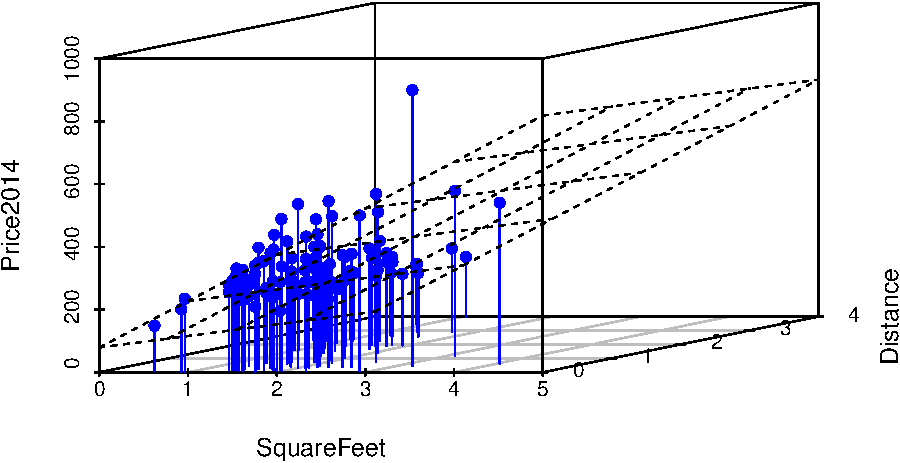
\includegraphics{09_InClass_Answers_files/figure-latex/unnamed-chunk-3-1.pdf}
\vspace{0.5 in}

\begin{longtable}[]{@{}llll@{}}
\toprule
& 1 mile & 2 miles & Difference\tabularnewline
\midrule
\endhead
1000 \(ft^2\) & 211.117 & 195.329 & -15.788\tabularnewline
\bottomrule
\end{longtable}

For every 1 additional mile away from the Rail Trail, the price of a
house in 2014 would decrease by \$15,788, on average, adjusted for house
size in square feet.

\newpage

\hypertarget{adjusting-for-distance-group}{%
\section{Adjusting for Distance
Group}\label{adjusting-for-distance-group}}

Rather than distance in miles, what if we thought a more useful measure
would be whether the house was closer (\textless{}1 mile from an
entrance to the rail trail) or further away (\(\geq\) 1 mile from a rail
trail entrance)?

\begin{itemize}
\tightlist
\item
  \texttt{Price2014}: Zillow price estimate from 2014 (in thousands of
  dollars)
\item
  \texttt{DistGroup}:

  \begin{itemize}
  \tightlist
  \item
    \texttt{Closer}: \textless{}1 mile to the nearest entry point to the
    rail trail network
  \item
    \texttt{Farther\ Away}: \(\geq\) 1 mile to the nearest entry point
    to the rail trail network
  \end{itemize}
\item
  \texttt{SquareFeet}: Square footage of interior finished space (in
  thousands of sf)
\end{itemize}

\texttt{R} treats \texttt{DistGroup} as a \texttt{factor} variable. It
can also be treated as a numeric variable, where one category has the
value of 0 and the other category has the value of 1. In other words,
you can think that the numerical equivalent is: ``Closer'' = 0 and
``Farther Away'' = 1.

\begin{Shaded}
\begin{Highlighting}[]
\NormalTok{m2<-}\KeywordTok{lm}\NormalTok{(Price2014 }\OperatorTok{~}\StringTok{ }\NormalTok{SquareFeet}\OperatorTok{+}\NormalTok{DistGroup , }\DataTypeTok{data =}\NormalTok{ RailsTrails)}
\KeywordTok{summary}\NormalTok{(m2)}
\end{Highlighting}
\end{Shaded}

\begin{verbatim}
## 
## Call:
## lm(formula = Price2014 ~ SquareFeet + DistGroup, data = RailsTrails)
## 
## Residuals:
##     Min      1Q  Median      3Q     Max 
## -136.55  -30.14   -2.14   22.17  321.40 
## 
## Coefficients:
##                       Estimate Std. Error t value Pr(>|t|)    
## (Intercept)              80.10      23.13   3.463 0.000785 ***
## SquareFeet              150.50      11.83  12.724  < 2e-16 ***
## DistGroupFarther Away   -36.97      13.51  -2.736 0.007356 ** 
## ---
## Signif. codes:  0 '***' 0.001 '**' 0.01 '*' 0.05 '.' 0.1 ' ' 1
## 
## Residual standard error: 64.59 on 101 degrees of freedom
## Multiple R-squared:  0.6673, Adjusted R-squared:  0.6607 
## F-statistic: 101.3 on 2 and 101 DF,  p-value: < 2.2e-16
\end{verbatim}

\textbf{\[\widehat{Price2014} = \hat{\beta}_0 + \hat{\beta}_1 \cdot SquareFeet + \hat{\beta}_2 \cdot Far\]}

\begin{enumerate}
\def\labelenumi{\arabic{enumi}.}
\tightlist
\item
  What price would this model predict for a 1000 square foot house that
  is \emph{Closer} from the rail trail?
\end{enumerate}

\(\widehat{Price2014} = 80.10 + 150.50 \cdot 1 -36.97 \cdot 0 =\) 230.6

\begin{enumerate}
\def\labelenumi{\arabic{enumi}.}
\setcounter{enumi}{1}
\tightlist
\item
  What price would this model predict for a 1000 square foot house that
  is \emph{Farther Away} from the rail trail?
\end{enumerate}

\(\widehat{Price2014} = 80.10 + 150.50 \cdot 1 -36.97 \cdot 1=\) 193.63

\begin{enumerate}
\def\labelenumi{\arabic{enumi}.}
\setcounter{enumi}{2}
\tightlist
\item
  What price would this model predict for a 2000 square foot house that
  is \emph{Closer} from the rail trail?
\end{enumerate}

\(\widehat{Price2014} = 80.10 + 150.50 \cdot 2 -36.97 \cdot 0=\) 381.1

\begin{enumerate}
\def\labelenumi{\arabic{enumi}.}
\setcounter{enumi}{3}
\tightlist
\item
  What price would this model predict for a 2000 square foot house that
  is \emph{Farther Away} from the rail trail?
\end{enumerate}

\(\widehat{Price2014} = 80.10 + 150.50 \cdot 2 -36.97 \cdot 1=\) 344.13

\begin{Shaded}
\begin{Highlighting}[]
\KeywordTok{library}\NormalTok{(moderndive)}
\KeywordTok{qplot}\NormalTok{(}\DataTypeTok{y=}\NormalTok{Price2014, }\DataTypeTok{x=}\NormalTok{SquareFeet, }\DataTypeTok{color=}\NormalTok{DistGroup, }\DataTypeTok{data=}\NormalTok{RailsTrails)}\OperatorTok{+}\KeywordTok{geom_parallel_slopes}\NormalTok{(}\DataTypeTok{se=}\OtherTok{FALSE}\NormalTok{)}
\end{Highlighting}
\end{Shaded}

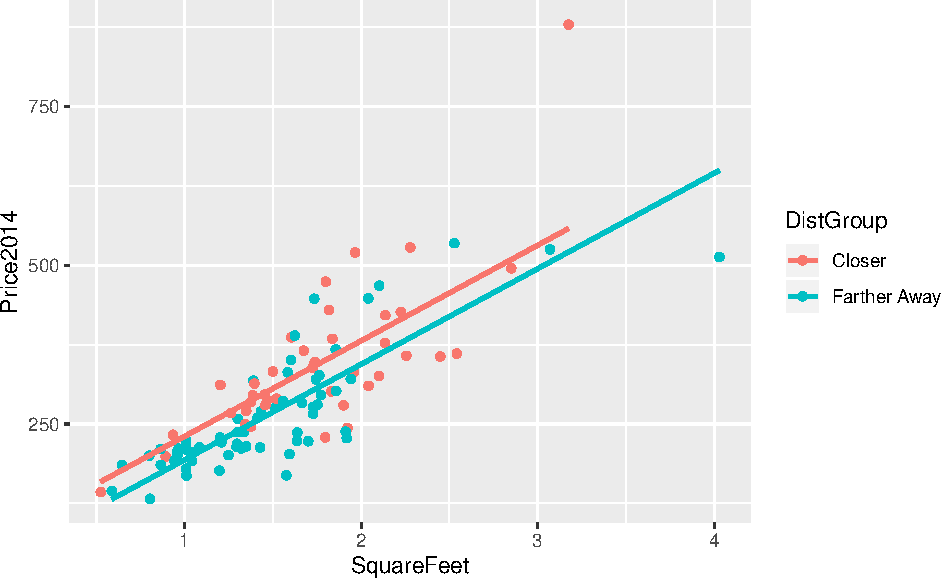
\includegraphics{09_InClass_Answers_files/figure-latex/unnamed-chunk-8-1.pdf}

\vspace{0.5 in}

\begin{longtable}[]{@{}llll@{}}
\toprule
\(ft^2\) & Close & Far & Difference\tabularnewline
\midrule
\endhead
1000 \(ft^2\) & 230.6 & 193.63 & -36.97\tabularnewline
2000 \(ft^2\) & 381.1 & 344.13 & -36.97\tabularnewline
Difference & 150.5 & 150.5 &\tabularnewline
\bottomrule
\end{longtable}

\textbf{For every additional 1000 \(ft^2\) of house size, our model
suggests the estimated 2014 price will increase, on average, by
\$150,500, adjusted for whether the house is closer or farther from the
rail trail.}

\textbf{On average, a house that is farther away from the rail trail
will be \$-36,970 less than a house closer to the rail trail, adjusted
for house size in square feet.}

The slope of the line is defined by the house size (\(ft^2\)); the
distance (far vs.~close) affects the intercept. So the lines have
parallel slopes, and the difference between two identically sized houses
where one is close and one that is far will always be the same amount
regardless of how big or small the house is.

\hypertarget{bedrooms}{%
\section{Bedrooms}\label{bedrooms}}

Rather than square feet, let's consider the number of bedrooms the house
has, in addition to its distance from the rail trail.

\begin{itemize}
\tightlist
\item
  \texttt{Price2014}: Zillow price estimate from 2014 (in thousands of
  dollars)
\item
  \texttt{BedGroup}: Categorical Variable of house type by group of
  bedrooms:

  \begin{itemize}
  \tightlist
  \item
    1-2 bedrooms (reference),
  \item
    3 bedrooms,
  \item
    4+ bedrooms
  \end{itemize}
\item
  \texttt{Distance}: Distance (in miles) to the nearest entry point to
  the rail trail network
\end{itemize}

You can think about \texttt{BedGroup} similarly to \texttt{DistGroup}
and consider the 3 bedroom group output in the model below akin to an
indicator variable with the values of 0 or 1: 0 if the house doesn't
have 3 bedrooms and 1 if it does have 3 bedrooms. Same for 4+ bedrooms.

\begin{Shaded}
\begin{Highlighting}[]
\NormalTok{m3 <-}\StringTok{ }\KeywordTok{lm}\NormalTok{(Price2014 }\OperatorTok{~}\StringTok{ }\NormalTok{Distance}\OperatorTok{+}\NormalTok{BedGroup, }\DataTypeTok{data =}\NormalTok{ RailsTrails)}
\KeywordTok{summary}\NormalTok{(m3)}
\end{Highlighting}
\end{Shaded}

\begin{verbatim}
## 
## Call:
## lm(formula = Price2014 ~ Distance + BedGroup, data = RailsTrails)
## 
## Residuals:
##     Min      1Q  Median      3Q     Max 
## -195.28  -48.15  -13.19   26.02  509.02 
## 
## Coefficients:
##                 Estimate Std. Error t value Pr(>|t|)    
## (Intercept)       283.56      26.67  10.633  < 2e-16 ***
## Distance          -42.30      10.18  -4.154 6.89e-05 ***
## BedGroup3 beds     39.88      26.63   1.498 0.137364    
## BedGroup4+ beds   106.13      28.49   3.725 0.000323 ***
## ---
## Signif. codes:  0 '***' 0.001 '**' 0.01 '*' 0.05 '.' 0.1 ' ' 1
## 
## Residual standard error: 93.12 on 100 degrees of freedom
## Multiple R-squared:  0.3153, Adjusted R-squared:  0.2948 
## F-statistic: 15.35 on 3 and 100 DF,  p-value: 2.746e-08
\end{verbatim}

\(\widehat{Price2014} = \hat{\beta}_0 + \hat{\beta}_1 \cdot Distance + \hat{\beta}_2 \cdot 3 Beds + \hat{\beta}_3 \cdot {4+} Beds\)

\hypertarget{mile-distance}{%
\subsection{1 mile Distance}\label{mile-distance}}

\begin{enumerate}
\def\labelenumi{\arabic{enumi}.}
\setcounter{enumi}{4}
\tightlist
\item
  What price would this model predict for a house 1 mile away that has
  1-2 Bedrooms?
\end{enumerate}

\(\widehat{Price2014} = 283.56 - 42.30 \cdot 1 + 39.88 \cdot 0 + 106.13 \cdot 0=\)
241.26

\begin{enumerate}
\def\labelenumi{\arabic{enumi}.}
\setcounter{enumi}{5}
\tightlist
\item
  What price would this model predict for a house 1 mile away that has 3
  Bedrooms?
\end{enumerate}

\(\widehat{Price2014} = 283.56 - 42.30 \cdot 1 + 39.88 \cdot 1 + 106.13 \cdot 0=\)
281.14

\begin{enumerate}
\def\labelenumi{\arabic{enumi}.}
\setcounter{enumi}{6}
\tightlist
\item
  What price would this model predict for a house 1 mile away that has
  4+ Bedrooms?
\end{enumerate}

\(\widehat{Price2014} = 283.56 - 42.30 \cdot 1 + 39.88 \cdot 0 + 106.13 \cdot 1=\)
347.39

\hypertarget{mile-distance-1}{%
\subsection{2 mile Distance}\label{mile-distance-1}}

\begin{enumerate}
\def\labelenumi{\arabic{enumi}.}
\setcounter{enumi}{7}
\tightlist
\item
  What price would this model predict for a house 2 miles away that has
  1-2 Bedrooms?
\end{enumerate}

\(\widehat{Price2014} = 283.56 - 42.30 \cdot 2 + 39.88 \cdot 0 + 106.13 \cdot 0=\)
198.96

\begin{enumerate}
\def\labelenumi{\arabic{enumi}.}
\setcounter{enumi}{8}
\tightlist
\item
  What price would this model predict for a house 2 miles away that has
  3 Bedrooms?
\end{enumerate}

\(\widehat{Price2014} =283.56 - 42.30 \cdot 2 + 39.88 \cdot 1 + 106.13 \cdot 0 =\)
238.84

\begin{enumerate}
\def\labelenumi{\arabic{enumi}.}
\setcounter{enumi}{9}
\tightlist
\item
  What price would this model predict for a house 2 miles away that has
  4+ Bedrooms?
\end{enumerate}

\(\widehat{Price2014} = 283.56 - 42.30 \cdot 2 + 39.88 \cdot 0 + 106.13 \cdot 1 =\)
305.09

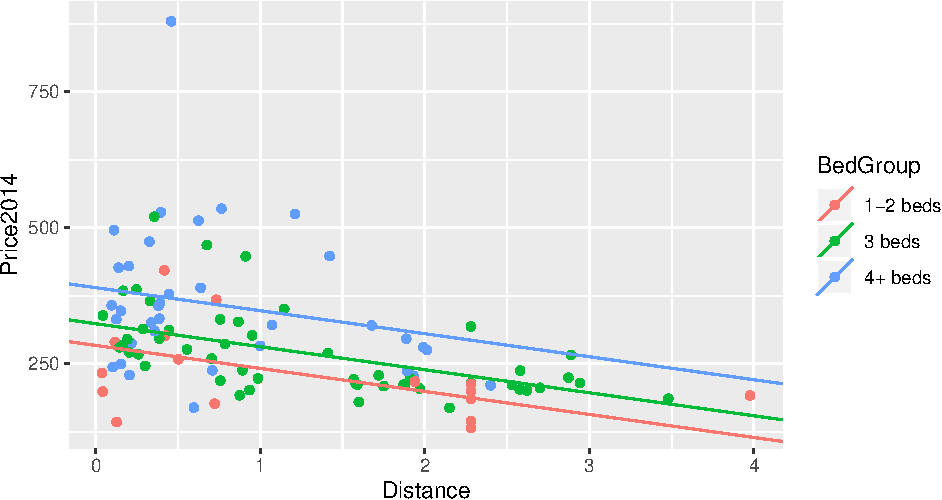
\includegraphics{09_InClass_Answers_files/figure-latex/unnamed-chunk-16-1.pdf}

\begin{longtable}[]{@{}llll@{}}
\toprule
Distance & 1-2 Beds & 3 beds & Difference\tabularnewline
\midrule
\endhead
1 mile & 241.26 & 281.14 & 39.88\tabularnewline
2 miles & 198.96 & 238.84 & 39.88\tabularnewline
Difference & -42.3 & -42.3 &\tabularnewline
\bottomrule
\end{longtable}

\begin{longtable}[]{@{}llll@{}}
\toprule
Distance & 1-2 Beds & 4+ beds & Difference\tabularnewline
\midrule
\endhead
1 mile & 241.26 & 347.39 & 106.13\tabularnewline
2 miles & 198.96 & 305.09 & 106.13\tabularnewline
Difference & -42.3 & -42.3 &\tabularnewline
\bottomrule
\end{longtable}

\textbf{Similar to the example above with a binary explanatory variable,
the bed group categorical variable also affects the intercepts, which
makes parallel lines for each of the three bedroom groups with the same
slope based on distance to the rail trail.}

\newpage

\hypertarget{back-to-distance-group}{%
\section{Back to Distance Group}\label{back-to-distance-group}}

What if we thought that the relationship between Square Footage of a
house and its price would \emph{vary} by whether it's closer or further
from the rail trail. A big house may not matter as much if it's really
far from the rail trail, and a smaller house may be more valuable if
it's closer to the rail trail than if it were further away.

You can also think about bigger houses in terms of an addition to a
house -- will adding another 500\(ft^2\) increase the value of your
price the same amount regardless of where the house is located, or do
you think that adding 500\(ft^2\) to a house close to the rail trail
will matter more/less for the total house's price than if the house were
further from the rail trail. Imagine you were a realtor and were asked
whether a homeowner should build an addition to their house -- how would
you respond?

\begin{Shaded}
\begin{Highlighting}[]
\NormalTok{m4 <-}\StringTok{ }\KeywordTok{lm}\NormalTok{(Price2014 }\OperatorTok{~}\StringTok{ }\NormalTok{SquareFeet}\OperatorTok{*}\NormalTok{DistGroup , }\DataTypeTok{data =}\NormalTok{ RailsTrails)}
\KeywordTok{summary}\NormalTok{(m4)}
\end{Highlighting}
\end{Shaded}

\begin{verbatim}
## 
## Call:
## lm(formula = Price2014 ~ SquareFeet * DistGroup, data = RailsTrails)
## 
## Residuals:
##      Min       1Q   Median       3Q      Max 
## -130.287  -32.792    0.084   23.018  282.596 
## 
## Coefficients:
##                                  Estimate Std. Error t value Pr(>|t|)    
## (Intercept)                         32.16      36.11   0.891   0.3752    
## SquareFeet                         177.82      19.75   9.003 1.51e-14 ***
## DistGroupFarther Away               32.46      42.57   0.763   0.4475    
## SquareFeet:DistGroupFarther Away   -42.15      24.53  -1.718   0.0889 .  
## ---
## Signif. codes:  0 '***' 0.001 '**' 0.01 '*' 0.05 '.' 0.1 ' ' 1
## 
## Residual standard error: 63.97 on 100 degrees of freedom
## Multiple R-squared:  0.6769, Adjusted R-squared:  0.6672 
## F-statistic: 69.82 on 3 and 100 DF,  p-value: < 2.2e-16
\end{verbatim}

\textbf{\[\widehat{Price2014} = \hat{\beta}_0 + \hat{\beta}_1 \cdot SquareFeet + \hat{\beta}_2 \cdot FartherAway + \hat{\beta}_3 \cdot (SquareFeet \times FartherAway)\]}

\begin{enumerate}
\def\labelenumi{\arabic{enumi}.}
\setcounter{enumi}{10}
\tightlist
\item
  What price would this model predict for a 1000 square foot house that
  is \emph{Closer} from the rail trail?
\end{enumerate}

\(\widehat{Price2014} = 32.16 + 177.82 \cdot 1 + 32.46 \cdot 0 - 42.15 \cdot 0=\)
209.98

\begin{enumerate}
\def\labelenumi{\arabic{enumi}.}
\setcounter{enumi}{11}
\tightlist
\item
  What price would this model predict for a 1000 square foot house that
  is \emph{Farther Away} from the rail trail?
\end{enumerate}

\(\widehat{Price2014} = 32.16 + 177.82 \cdot 1 + 32.46 \cdot 1 - 42.15 \cdot 1=\)
200.29

\begin{enumerate}
\def\labelenumi{\arabic{enumi}.}
\setcounter{enumi}{12}
\tightlist
\item
  What price would this model predict for a 2000 square foot house that
  is \emph{Closer} from the rail trail?
\end{enumerate}

\(\widehat{Price2014} = 32.16 + 177.82 \cdot 2 + 32.46 \cdot 0 - 42.15 \cdot 0=\)
387.8

\begin{enumerate}
\def\labelenumi{\arabic{enumi}.}
\setcounter{enumi}{13}
\tightlist
\item
  What price would this model predict for a 2000 square foot house that
  is \emph{Farther Away} from the rail trail?
\end{enumerate}

\(\widehat{Price2014} = 32.16 + 177.82 \cdot 1 + 32.46 \cdot 1 - 42.15 \cdot 2=\)
335.96

\newpage

\begin{Shaded}
\begin{Highlighting}[]
\KeywordTok{qplot}\NormalTok{(}\DataTypeTok{y=}\NormalTok{Price2014, }\DataTypeTok{x=}\NormalTok{SquareFeet, }\DataTypeTok{data=}\NormalTok{RailsTrails, }\DataTypeTok{color=}\NormalTok{DistGroup) }\OperatorTok{+}\StringTok{ }
\StringTok{  }\KeywordTok{geom_smooth}\NormalTok{(}\DataTypeTok{method=}\NormalTok{lm,}\DataTypeTok{se=}\OtherTok{FALSE}\NormalTok{,}\DataTypeTok{fullrange =} \OtherTok{TRUE}\NormalTok{)}
\end{Highlighting}
\end{Shaded}

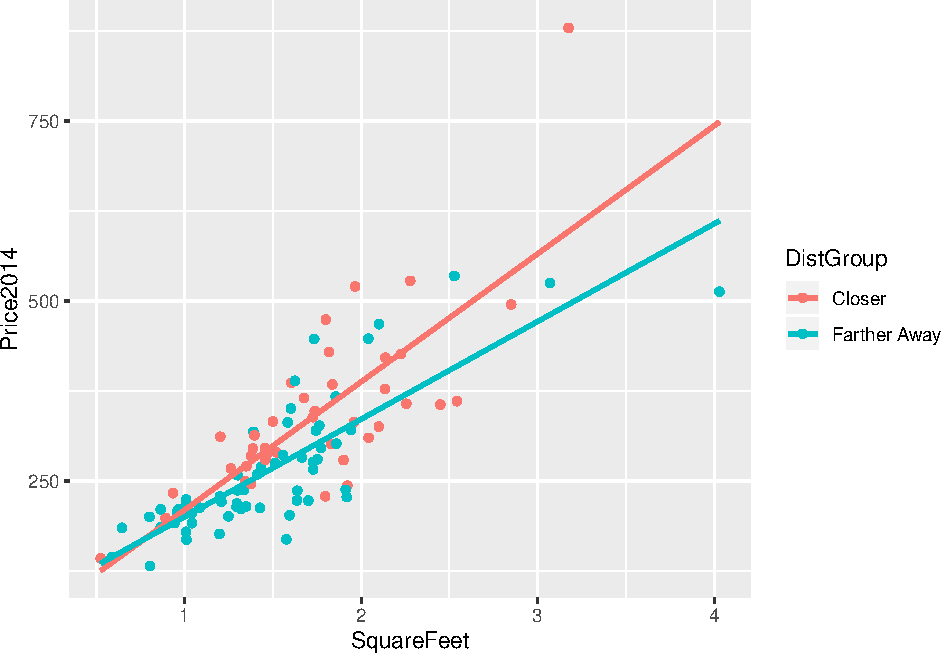
\includegraphics{09_InClass_Answers_files/figure-latex/unnamed-chunk-22-1.pdf}

\vspace{0.5 in}

\begin{longtable}[]{@{}llll@{}}
\toprule
\(ft^2\) & Close & Far & Difference\tabularnewline
\midrule
\endhead
1000 \(ft^2\) & 209.98 & 200.29 & -9.69\tabularnewline
2000 \(ft^2\) & 387.8 & 335.96 & -51.84\tabularnewline
Difference & 177.82 & 135.67 &\tabularnewline
\bottomrule
\end{longtable}

\textbf{The model suggests that the relationship between SquareFeet and
Price varies by whether the house is close or far from the rail trail.
(This difference is not statistically significant, but let's not worry
about that for now; let's just think about the coefficients and what
they are telling us separate from their hypothesis tests.)}

The \(\hat{\beta}_2 Far\) variable affects the intercept. A house that
has 0 square feet and is far from the rail trail will be worth
\$32,458.25 more than a house of the same size that is closer.

For every additional 1000 \(ft^2\) of house size, our model suggests the
estimated 2014 price will increase, on average, though at different
rates depending on whether the house is close or far from the rail
trail. Houses far from the rail trail will increase more slowly in price
as they have more square footage than houses closer to the rail trail
do.

For every additional 1000 \(ft^2\) in size, the price of a house that is
\emph{close} to the rail trail will, on average, increase by
\$177,818.2.

For every additional 1000 \(ft^2\) in size, the price of a house that is
\emph{far} to the rail trail will, on average, increase by \$135,669.1.

The \emph{marginal difference} in the house price for each 1000 square
feet between houses that are far versus those that are closer is, on
average, \$-42,149.1

\end{document}
